\section{Knowledge base}

\subsection{Print preparations}

The term \emph{print preparation} summarizes information about:

\begin{itemize}
  \item Determining material properties

    \begin{itemize}
      \item Material specific extrusion temperature
      \item Finding the extrusion multiplier
      \item Filament quality
    \end{itemize}

  \item 3D-suitable construction and slicing
    \begin{itemize}
      \item Handling 3D-files
      \item Layers and quality
      \item Dimensional accuracy
    \end{itemize}

\end{itemize}

and the like, which may be useful or required prior to printing. 

\subsubsection{Setting the extrusion temperature}

Depending on the material and even with the same but differently colored material the extrusion temperature varies strongly. Most manufacturers provide suggestions for their materials which are always a good idea to start with when printing a new material for the first time.

Fine-tuning the temperature can improve results or reduce unwanted side effects (such as oozing and stringing). Some materials react astonishingly different within a temperature range of $\pm$ 5\degree C. For this reason the GUI of the HT500.3 is equipped with a direct temperature control and extrude function for quick-and-easy evaluating different temperature settings.

\begin{figure}[H]
  \centering
  \includegraphics[width=.7\linewidth]{./img/gui_expertmenu_2_v110.png}
  \caption{Try finding the suitable temperature by directly extruding via the 
           \emph{Expert Control} screen.}
\end{figure}

\begin{info}
  Observe that the temperature shown in the footer of the GUI is measured at the hot end heater and may be 5 - 10\degree C lower at the nozzle tip. Try increasing the temperature if you are discontented by the printing results.

  When extruding new materials do not forget to examine the calibration of the correct extrusion multiplier.

  When no filament profile is active for the extruder, the starting temperature 
  is set as 180\degree C.
\end{info}

To find a suitable extrusion temperature: 

\begin{enumerate}
  \item Open the \emph{Expert Control} menu.
        On the right hand side of the screen you will find buttons to choose the extruder (left or right).
  \item Choose an extruder.
        After selecting ([Left]/[Right]) the menu is extended. The starting temperature is displayed according to the selected filament profile (see Configuration).
  \item Enter the extrusion temperature recommended by the manufacturer via 
        the touchscreen keyboard. The temperature can be increased or decreased in steps of
        10\degree C (tap [++] / [- -] once) or 1\degree C (tap [+] / [-] once).
  \item Tap [set] when the desired value is set.
        The 3D printer will heat to this temperature and then unlock the [extrude] and [retract] buttons.
  \item Tap [extrude] to extrude 5 mm of filament 
        (tapping repeatedly will extrude 5 mm per tap). Tapping [retract] pulls the filament 5 mm back for every tap.
  \item Watch the extrusion and check whether the following recommendations are visible:
    \begin{enumerate}
      \item The filament is extruded smoothly in a single, clean strand.
      \item No bubbling or discoloration is visible. Bubbling or discoloration 
            mean an \emph{extrusion temperature set too high}.
            If bubbling does not cease after reducing the temperature, this may also mean that the material absorbed moisture. It must then be dried thoroughly.
      \item The extruded strand is not swelling up after leaving the nozzle tip. 
            Upswell means the temperature is too low and the internal friction of the material too high.
      \item No slipping of the extruder drive gear is visible. Slipping of the drive gear 
            indicates an extrusion temperature set too low and a too high frictional resistance in the nozzle.
      \item The material is not oozing excessively from the nozzle tip after 
            finishing the extrusion and reducing the temperature. \newline \newline
            If these points are not met, adjust the temperature and extrude again until the correct appearance is visible.
    \end{enumerate}
  \item Tap [OFF] to deactivate the extruder heating unless you want to keep the 
        current extruder temperature for further steps.
  \item To verify the settings, print a sample model and check the extrusion properties. 
        Adjust the settings if required.
\end{enumerate}


\subsubsection{Handling 3D files}

Any information we gather related to improving or easing the slicing process is listed in the following paragraphs. 


\paragraph{Easy evaluation of STL-files}

Especially when using files downloaded from open internet sources it may be that these files are not suitable for printing due to export or modeling mistakes. Misaligned edges (non-manifolds) and holes can render a 3D-model unprintable and make troubleshooting on the 3D-printer an infinite displeasure because no obvious reason can be detected.

One quick and simple way to eliminate this as an error source is checking the suitability of your STL-file for 3D-printing. All you need is a program capable of analyzing the STL-file's mesh.
Slic3r itself can deal with minor troubles. Other tools may be helpful as well to recognize a corrupted file. 

\paragraph{Slic3r part info:}

(see Slic3r manual also)
After opening a file in Slic3r, the info box in the bottom-right corner of the plater shows information on the model status. For a single, suitable part the info must look like:
\emph{Facets: xxxxx (1 shells)}
\emph{Manifold: Yes}

\begin{figure}[H]
  \centering
  \includegraphics[width=.7\linewidth]{./img/slic3r_brokenpart-analysis.png}
  \caption{Slic3r info box for a flawless (above) and a corrupted (below) part.}
\end{figure}

If it displays \emph{Manifold: Auto-repaired (xxxx errors)} the file contains degenerations.
It is most likely that it also shows an increased number of shells (e.g. \emph{Facets: xxxxx (6 shells)} because the part has been split.
Also check the 3D-preview for visible defects. In this case it is better to repair or reconstruct the model.
Regard that the auto-repair function of Sic3r is only suited for repairing minor defects.
Slic3r info box for a flawless (above) and a corrupted (below) part.


\paragraph{Overhang - adjusting the layer thickness}

If you want to print filigree objects with overhanging structures without adding supports, try reducing the layer thickness for this print by 15 - 20\%. This will result in a finer Z-axis resolution and increased overlay of subsequent layers so that more stability is gained over the height of the target object. 

\paragraph{Modifying infill and perimeters}

There are currently two Slic3r profiles available at our GitHub repository that provide preset ready-to-print slicing settings. Her are some tips for handling these profiles to adjust them to your needs.
The \emph{SOLID} profile normally needs no modification since it comes with stable, reliable settings for printing solid objects with 100 \% infill.
The \emph{ECO} profile supplies settings for objects with loosened infill. This makes objects lighter and reduces the print time and the material consumption. To achieve good results, the settings may have to be adjusted.
We recommend to set the following always for printing ECO objects: 

\begin{itemize}
  \item A hull thickness of 1.0 to 1.5 mm. As a rule of thumb divide the hull thickness by 
        he nozzle tip diameter and set the amount of perimeters equal to the result. Such, a closed, smooth and stable hull is ensured.
  \item Gyroid infill as it provides highest stability at optimal density.
  \item A minimum infill of 15 \%.
  \item A maximum infill of 45 \%. 
        Increasing the infill further does not have a significant advantage compared to a solid body.  
\end{itemize}


\subsubsection{Layers and quality}

If it comes to high-quality printing, there is no way to avoid grappling with the “layers” topic. The layer settings influence the quality of a print in the same way as extrusion temperature and movement speed do. In fact, all of these settings interact and influence one another, but you may have recognized that in every slicing software there are a lot of layer-specific settings waiting for adjustment.

The following paragraphs are meant to give you an overview on the topic and further to provide you with detailed information about necessary basic and useful advanced settings to stepwise increase your prints with the HT500.3.
As previously mentioned in this manual, we are focused on printing ABS as a reference so the following mostly refers to settings with this material; if otherwise, it will be specially emphasized.
When talking about software settings we always refer to the Slic3r Prusa Edition software.

Everything else only refers to printing with the HT500.3, since this is the basis of our experience. Most things may also be valid for other appliances and different slicing software since it is basic knowledge about FFF manufacturing which can be found elsewhere in books and on the internet. We want to enable the user of a HT500.3 to achieve the best possible results with his machine and to provide the necessary knowledge from a single source. 

\paragraph{Warping prevention}

One of the most important factors deciding whether a print finishes at all and if it does defining the final quality is the adhesion of the first layer to the print bed. The first layer channels off heat tensions from the printed object into the print bed.
ABS, Polycarbonate and Nylon for example are very prone to warping, so only firm adherence to the subsurface can effectively prevent bending and warping. With a first layer not sticking to the subsurface all-over, tensions will manifest all through the model - the object will detach itself from the print bed and the print is wasted. High temperature effected tensions manifest ever stronger with increasing height of the printed model. Long, straight perimeters enhance this effect further.
Three factors determine the adhesion: 

\begin{enumerate}
  \item A correctly leveled print bed (explained under \emph{Tips \& Tricks}), 
  \item the material of the print bed and 
  \item the temperature of the print bed. 
\end{enumerate}

The material of the print bed must match the chosen filament. The standardized PEI print beds delivered with the HT500.3 perfectly match the requirements for printing \emph{ABS} and 
\emph{HIPS}, the most common printing materials for this 3D printer. Other materials such as 
\emph{PET Copolyester} and \emph{TPE-u} also stick to the PEI surface unproblematically.

The most necessary print setting apart from the material is the correct print bed temperature to ensure that the filament sticks to its subsurface throughout the printing process. Some materials, like ABS or PC, need high temperatures to stick, whereas for others, such as Nylon or PVA, heat is counter-productive and a cold bed might be needed.

Other Slic3r settings that help minimizing warping are described in the \emph{Tips \& Tricks}section. 

\paragraph{The first layer}

One thing that always stands out when preparing a print job with the slicing software are the \emph{first layer} settings. While everything thereafter is only “layers”, the first layer is especially important for the result of any print job.
This is because of the requirements imposed on the first layer: 

\begin{itemize}
  \item Compensation of unevennesses of the subsurface to build an even foundation for the 
        following layers. Slight leveling mistakes, scratches and bends can provide quite an uneven underground; in the slicing profiles provided at our \emph{GitHub repository} the first layer is preset to be thicker and wider (see \emph{below}) than the following layers. The increased throughput during printing the first layer fills in waviness of the subsurfaces and thus provides an even underground for the following layers.
  \item Sticking to the print bed during the entire print job so that heat tensions are 
        channeled off and warping is minimized. The adherence to the print bed is above all responsible for the minimization or manifestation of warpage. Correct first layer settings become the more important the larger the printed object is and the more long, strung-out edges it contains.
  \item Loosing the adhesion after completion of the print job. After finishing a print job,
        the model must be detached from the print bed without breaking apart so the first layer must not merge permanently with the print bed but reversible (e.g. due to cooling). This is the only feature that cannot be influenced via the slicing settings and is totally dependent on the material match of printed plastic and print bed.
\end{itemize}

It has been a challenge to find materials matching the properties of ABS and the above named special features. After a lot of testing, we found that our PEI print bed meets all requirements concerning rigidity, stiffness, flatness, and thermal stability. In combination with the heating of the build chamber we experience no trouble printing straight, non-deforming objects and have had no problems so far removing our models from the print bed.
If you are sure to have leveled your print bed correctly and all temperatures are set right and still you experience delamination and warpage, have a look at your first layer settings; there might be something to be improved here. 


\paragraph{First layer settings}

As mentioned above, the following recommendations are valid for printing ABS on the HT500.3. We have taken all this into respect when creating our slicing profiles and you do not need to try and find matching settings for the first prints. After growing accustomed to 3D printing and the apparatus' specific features you can start optimizing. Also, if you want to print other materials than ABS, the basic settings named here apply and can be used to modify your results.
The first layer should be thicker and wider than the following layers. In case of the HT500 we recommend the following (and have already taken it into respect in our slicing profiles):

\begin{info}
The following applies to the nozzle tip size 0.35 mm and the preset Slic3r profiles you installed during initial commissioning. It is meant to give you an overview of the settings relevant for the optimization of the first layer adhesion. Please experiment to find the settings best suited for your task and test all settings before applying them to your final model if you use other nozzle sizes.
When using the 0.5 or the 0.75 mm nozzle tip, there is no further improvement when setting the layer height equal to the nozzle tip diameter. A value of 0.4 mm will suffice for these nozzle tips. 
\end{info}

\begin{itemize}
  \item The first layer height should be adequate to the nozzle tip's diameter.
        For example:
        Printing with a nozzle tip size 0.35 
        means setting the first layer height to \emph{0.35 mm}

    \begin{figure}[H]
      \centering
      \includegraphics[width=.7\linewidth]{./img/slic3r_firstlayersettings.png}
      \caption{Slic3r Print Settings - setting the first layer height}
    \end{figure}

  \item The extrusion width should be set to 150 \% of the first layer height.
        For example:
        Printing with a nozzle tip size 0.35 and thus 0.35 mm first layer height, setting the first layer extrusion width to 150 \% means an extrusion width of 0.53 mm. This ensures that enough filament is extruded to compensate for slight unevenness of the subsurface and still enough adhesion.
        In Slic3r you can preset and save this setting as a percentage so that the first layer's extrusion width is independent of the actual nozzle tip size.

    \begin{figure}[H]
      \centering
      \includegraphics[width=.7\linewidth]{./img/slic3r_advancedsettings.png}
      \caption{Slic3r Advanced Settings - reducing the first layer extrusion width}
    \end{figure}
    
    \begin{info}
      Both above mentioned measures compensate for unevennesses of the print bed and increase the tolerance against slight leveling mistakes. The distance between nozzle tip and print bed will assure that the bore is not clogged when passing convex bumps by leaving enough free space in between. The extrusion width will make sure that enough material is conveyed to equalize concave crudities.
    \end{info}

  \item The first layer speed should be reduced because the print bed does not fuse easily 
        with the material. Slower movement ensures a more even temperature distribution between underground and material and thereby a better binding between them as well as longer cooling time which aids relaxation of tensions.
        For ABS, a first layer speed of \emph{15 mm/s} is a functional value. For other materials, settings from 10 to \emph{30 mm/s} are recommended 
        (always choose slower values for nozzle tips $\leq$ 0.35 mm). 

    \begin{figure}[H]
      \centering
      \includegraphics[width=.7\linewidth]{./img/slic3r_firstlayerspeed.png}
      \caption{Slic3r Print Settings - setting the first layer extrusion speed}
    \end{figure}

  \item Changing the extrusion temperature and the print bed temperature can also improve 
        the first layer adherence. Changing the temperature a few degrees may allow for the filament to melt a little more inviscid and to lay more evenly onto the print bed.
        Increasing the print bed temperature can have a similar effect as reducing the extrusion speed: a better temperature distribution and increased cooling time.
        For printing ABS we find no difference in quality using varying temperatures so the settings are the same for the first and the following layers but this feature may help printing other plastics.
    \begin{info}
      Optimize the extrusion and print bed temperature for the Material currently installed.
      Do not hesitate to try different settings here, since even colored additives may alter the optimal extrusion temperature.
    \end{info}

  \item For filigree or thin-walled objects add a 3 to 6 mm brim and/or 3 to 8 raft layers 
        to increase the effective adhering area. 

    \begin{figure}[H]
      \centering
      \includegraphics[width=.7\linewidth]{./img/slic3r_brim.png}
      \caption{Slic3r Print Settings - adding a brim}
    \end{figure}

  \item Adding a raft may also compensate leveling mistakes. 

    \begin{figure}[H]
      \centering
      \includegraphics[width=.7\linewidth]{./img/slic3r_raft.png}
      \caption{Slic3r Print Settings - adding raft layers}
    \end{figure}

\end{itemize}

These are the settings for the first layer. Try and experiment with them to improve your results or to print new materials. We shall do the same and publish all relevant findings.

\paragraph{Adhesion faults} 

The fault easiest to diagnose and remedy is the presence of abhesives on the print bed. Recently removed an object from the print bed? Maybe touched the surface? Fingerprints are very effective separating agents that will with certainty prevent sticking of the filament. Any oil, fat, grease or the like will have this effect, so make sure you always \emph{clean} the print bed with a suitable solvent before starting a new print.

In most cases, \emph{false leveling} of the print bed is the reason for unsatisfactorily adhesion of the first layer. If the distance between the print bed surface and the nozzle tip becomes to wide, the filament will not be pressed but laid on the surface and single strands will not merge. No cohesion between adjoined strands and no adherence to the underground will develop. It is easy to recognize and as easy to correct such faults as result from false leveling.
Too low a temperature of the print bed also effects poor first layer adhesion. In such cases it might be necessary to find the correct temperature by simply trying. If you cannot succeed with this, something might be wrong with the heating element. 


\paragraph{Following layers}

Whereas the first layer decides if a print can be finished or not, the following layers influence the fineness and optical appearance of the model. Thinner layers improve the surface quality and chamfers and curvatures are more refined and smooth with much less visible steps. But choosing a lower layer height will also increase the printing time. Regard that halving the layer height more than doubles the print time and at some point the improvement of the appearance will be no longer visible. The other way around you will receive a rougher surface in a shorter time. It is depending on your demands which resolution you try to achieve and how much time you are able or willing to invest for a certain result. The slicing settings are not limited in this regard, so feel free to try it out.

We recommend the following settings when printing ABS or other viscous materials: 

\begin{itemize}
  \item The minimal layer height should not undercut \emph{0.1 mm}. 
        For values below this we have 
        no adequate experience since the improvement in surface resolution stands way behind the increase of print time. More inviscid materials may allow even thinner layers.
        Regard that the layer height is not necessarily limited by the nozzle tip diameter; it is possible to receive excellent results printing 0.1 mm layers with a 0.35 mm nozzle tip. In the same regard take note that the layer height does not implicitly improve every result. When it comes to fine structures and sharp edges, choosing a smaller nozzle tip without reducing the corresponding layer height can be the key to success.
  \item The maximal layer height should not exceed 80 \% of the nozzle tip diameter. Above 
        this value the distance between nozzle tip and previous layer becomes too far and the extruded amount of material may not suffice for good layer binding and thus strong, stable objects.
        Slicing software like Slic3r do allow configuring layer heights up to the actual nozzle tip diameter (100\%) but broad experience in FFF 3D printing shows, that max. 80\% is a safe approximate value for best results.  
\end{itemize} 


\subsubsection{Dimensional accuracy}

Dimensional accuracy is a core demand of any manufacturing process and therefore is a feature very much looked into in the HT500.3 3D printer. It is built to provide high mechanical accuracy in positioning and supports a variety of possibilities to compensate for mechanical influence factors to improve appearance and dimensional accuracy.
Also, the recommended slicing software \emph{Slic3r Prusa Edition} calculates extrusion width, material flow and movement to precisely match the dimensions given in the .stl-file.
Kühling\&Kühling aim to meet accuracy demands of $\pm$0.2 mm “out-of-the-box”, thus delivering every HT500.3 3D printer carefully adjusted and optimally calibrated.
But some factors that influence the dimensional accuracy of print objects cannot be compensated by the apparatus or the slicing software but can be partly neutralized by slightly altering the model geometry of the CAD-file.
Currently, it is not possible to compensate all influences equally and at the same time but the following tips provide some means to improve the dimensional accuracy of your prints if required. 

\paragraph{Influence of thermal expansion}

Any material is subject to thermal expansion when heated and shrinkage when cooled. Since the temperature range a plastic passes through during a print is very wide, reaching from around 100\degree C at the print bed surface to approx. 20\degree C when taken out of the build chamber, the influence of thermal expansion cannot be neglected. Thermoplastics usually have a relatively high thermal expansion factor.
For example: the thermal linear expansion coefficient $\alpha$ L of ABS 
is approximately $1\times 10^{-4}$ $K^{-1}$, which means that a part of 25 mm length (or diameter) will shrink by approximately:

$25 mm \times 1\times10^{-4} K^{-1} \times (100\degree C - 20\degree C) = 0.19 mm (\cong 0.76 \%)$

due to thermal influences alone.

A series of over two hundred measurements with printed ABS test bodies has shown that the effective deviation lies above the expected value, between 1 and 2\%, increasing with decreasing size. Especially for small dimensions $\leq$5 mm other effects 
(see below) may counter or intensify the deviation.
For nominal values between 2.5 and 25 mm, the deviation was measured for uncompensated test bodies and two different methods of compensation.
For the uncompensated measurements the above said applies.

The first and more complicated method of compensation is to directly apply the thermal expansion factor in the 3D CAD model and producing an .stl-file that already comes with corrected dimensions. This is only applicable if the 3D CAD program you are using provides the possibility to multiply all dimensions with a specific factor at once.
This method is advantageous if you want to check dimensions in the CAD-file, which is much more common for .stl-data than ready-sliced g-codes.

The second, more comfortable way is to directly upscale the model in Slic3r.
For that: 

\begin{itemize}
  \item Upload your .stl-file to Slic3r.  
  \item Choose the [Scale…] button and enter the percental scaling factor. 
\end{itemize} 

\begin{figure}[H]
  \centering
  \includegraphics[width=.7\linewidth]{./img/slic3r_upscale.png}
  \caption{Scaling the model directly in Slic3r.}
\end{figure}

A factor of 101 \% has proven to reduce thermal induced deviation to values between 0.15 and 0.75 \% for values $\geq$5 mm. 


Excerpt from the measurement report: 

\begin{table}[H]
  \centering
  \begin{tabulary}{\textwidth}{ L L L L L L L}
    \toprule
    Nominal \newline
    value 
      & Mean value \newline 
      (12 measurements) 
      & Deviation   
        & Compensated \newline
          via 3D CAD model \newline
            ($dim \times \alpha$ L) 
            & Deviation     
              & Compensated \newline
                via \newline
                Slic3r (101\%) 
                & Deviation    \\
    \lbrack mm  \rbrack
      & \lbrack mm  \rbrack   
      & \lbrack \%  \rbrack   
        & \lbrack mm  \rbrack   
          & \lbrack \%  \rbrack      
            & \lbrack mm  \rbrack
              & \lbrack \%  \rbrack          \\
    \midrule
    25.00     
      & 24.74   
        & 1.04    
          & 25.05   
            & 0.19    
              & 24.99          
                & 0.03          \\
    20.00     
      & 19.77   
        & 1.17    
          & 19.96   
            & 0.20    
              & 19.97   
                & 0.16          \\
    15.00     
      & 14.75   
        & 1.64    
          & 14.91   
            & 0.62    
              & 14.89   
                & 0.71          \\
    10.00
      & 9.84  
        & 1.65    
          & 10.03   
            & 0.30    
              & 9.97  
                & 0.27          \\
    5.00    
      & 4.94  
        & 1.18    
          & 4.99  
            & 0.30    
              & 4.98  
                & 0.50          \\
    2.50    
      & 2.40  
        & 4.20    
          & 2.44  
            & 2.40    
              & 2.45  
                & 1.93          \\
    \bottomrule
  \end{tabulary}
\end{table}

\begin{figure}[H]
  \centering
  \includegraphics[width=.7\linewidth]{./img/cylindric_pyramid_mean-values.png}
  \caption{The deviation decreases significantly when the thermal expansion is compensated.
           Either for diameters of circular structures …}
\end{figure}

\begin{figure}[H]
  \centering
  \includegraphics[width=.7\linewidth]{./img/cubic_pyramid_mean-values.png}
  \caption{… or linear dimensions.}
\end{figure}

The table above outlines that the improvement by either method is significant compared to the uncompensated model while not making much of a difference compared among each other.
All measurements where done for a set of twelve individually printed test bodies (see adjacent picture). The deviations of each set and diameter where averaged for comparison.
The table also shows that for smallest structures the effect is in fact significant but that other effects need compensating measures too to receive best results. 

\begin{figure}[H]
  \centering
  \includegraphics[width=.7\linewidth]{./img/pyrcompuncomp.png}
  \caption{visualization of the ABS test bodies printed for comparison and 
           evaluation. On the left hand-side the uncompensated model, on the right-hand side the model after multiplying with $\alpha$L prior to exporting the .stl.}
\end{figure}

\paragraph{Small holes}

Small hole dimensions may be subject to one additional error apart from shrinkage. 

A minor aspect is the number of triangles a model is built from, i.e. the number of facets. Normally, any .stl's resolution is fine enough for sufficiently reflecting the details of a model and respectively loss of accuracy is neglectable.
Still, for small bores the number of facets may play a role if it is very low.
The graphic on the right displays the possible influence of facets on an inner diameter.
In case of roughly faceted objects try increasing the resolution of your CAD model to improve dimensional accuracy. 


\begin{figure}[H]
  \centering
  \includegraphics[width=.7\linewidth]{./img/diameterdeviationextrusion2.png}
  \caption{Correlation of low faceted walls and diameter.}
\end{figure}


\subsubsection{Filament quality check}

Much to our regret, filament manufacturing is not subject to standardization yet. Although we try to provide material of high quality and stable dimensions, manufacturing faults cannot be totally excluded.
If you order filament of other suppliers, please check back that it is within the stated tolerances.
If you note that material purchased via Kühling\&Kühling does not meet the standards we set here, please let us know and we will promptly replace the material. We only ask you to send back the flawed material (return note will be included in the new delivery) so that we can discuss the matter with our supplier. 

If you experience increased problems with grinding at the drive gear, first thing to check is the quality of the filament currently loaded:

\begin{itemize}
  \item Is the diameter correct? 
  \item Is the filament round? 
  \item Is the filament free of bulges and kinks? 
\end{itemize}

\begin{info}
  To make sure that there is no problem in the filament feed system, try the following:
  \begin{itemize}
    \item Remove the filament feed hose from the filament inlet (push the blue fixing ring 
          and pull the hose out).
    \item Feed the filament directly through the hose and try printing.
          If the problem remains, check the filament as described.
  \end{itemize}

  Refit the hose afterwards!
\end{info}

\paragraph{Diameter}

Measure the diameter at several points (at least 5 per 0.5 m).
Measure at least twice (best thrice) at each point at an angle of 90\degree (60\degree). The diameter must not deviate from 

1.75$\pm$0.05 mm (1.70 … 1.80 mm)

A diameter of e.g. 1.90 mm will increase friction in the filament feed system and the nozzle barrel and cause compression and jamming of the filament.
A diameter of 2.00 mm will no longer fit through the filament feed inlet.

Filament below 1.70 mm is, especially when a print job requires a lot of retraction movement, likely to jam the nozzle barrel because molten filament can push itself back up the barrel and form a plug. 

\begin{figure}[H]
  \centering
  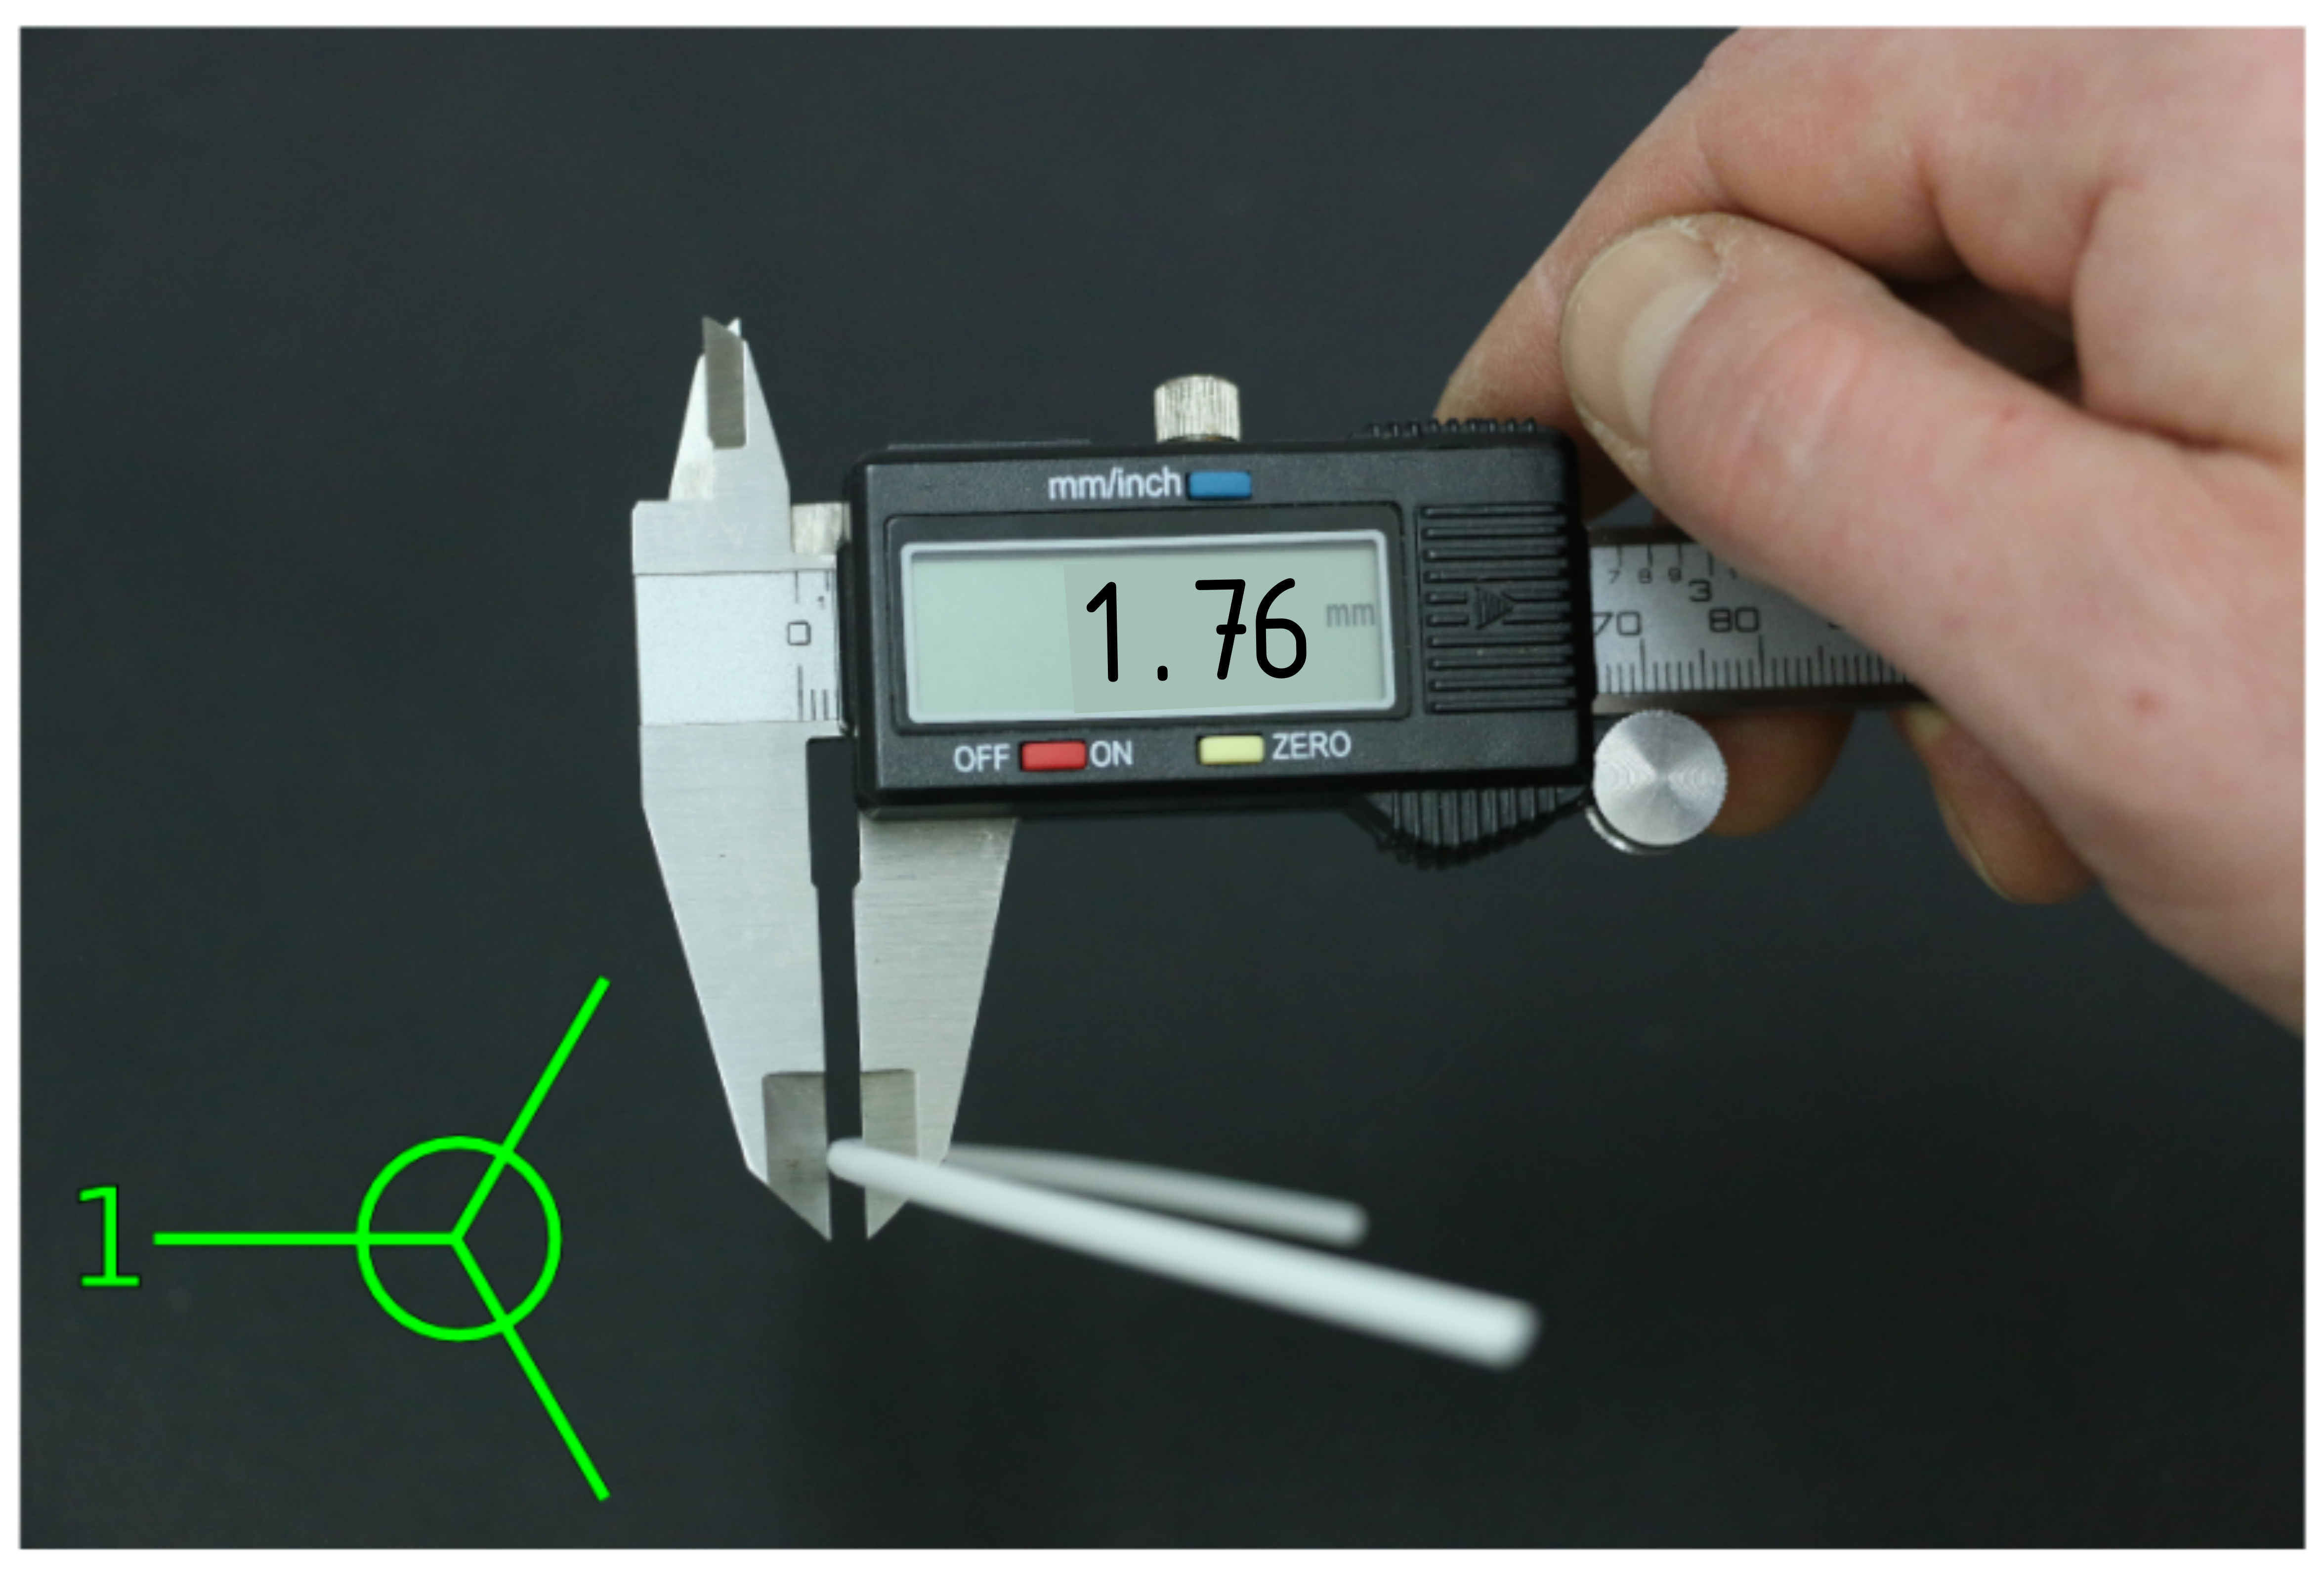
\includegraphics[width=.7\linewidth]{./img/filametmeasurediam_1.png}
  \caption{First measured diameter.}
\end{figure}


\begin{figure}[H]
  \centering
  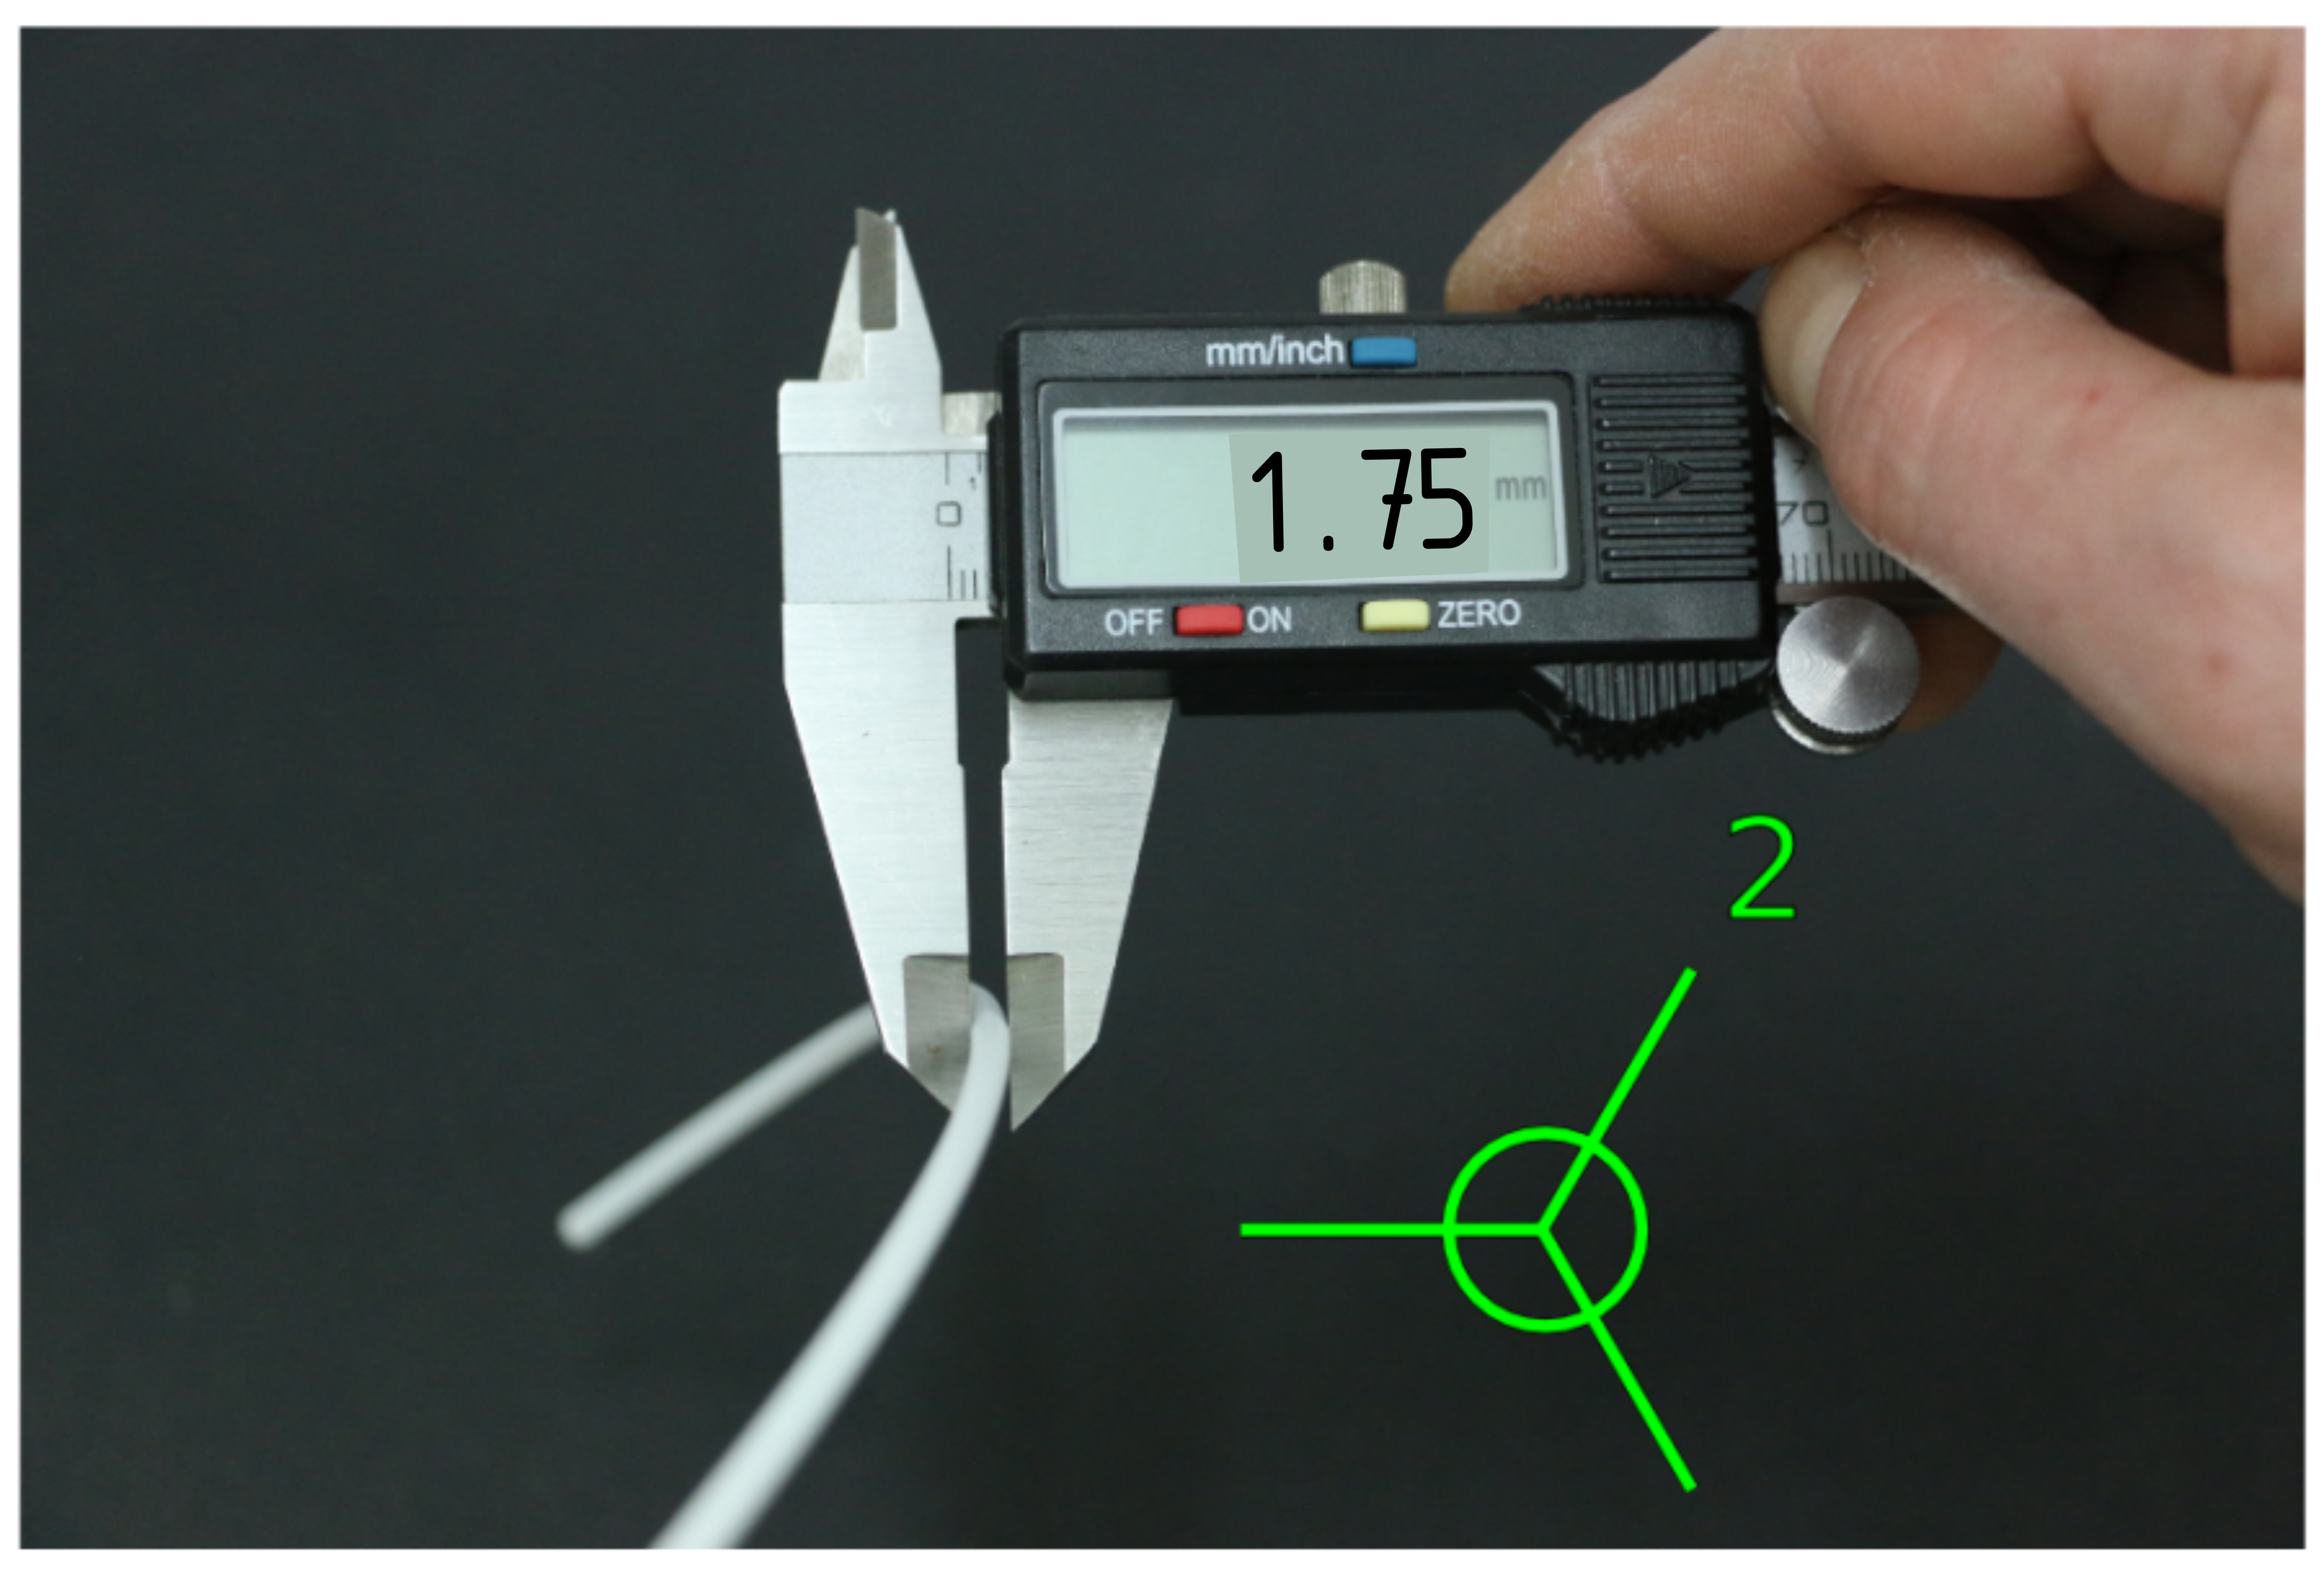
\includegraphics[width=.7\linewidth]{./img/filametmeasurediam_2.png}
  \caption{Second measured diameter.}
\end{figure}


\begin{figure}[H]
  \centering
  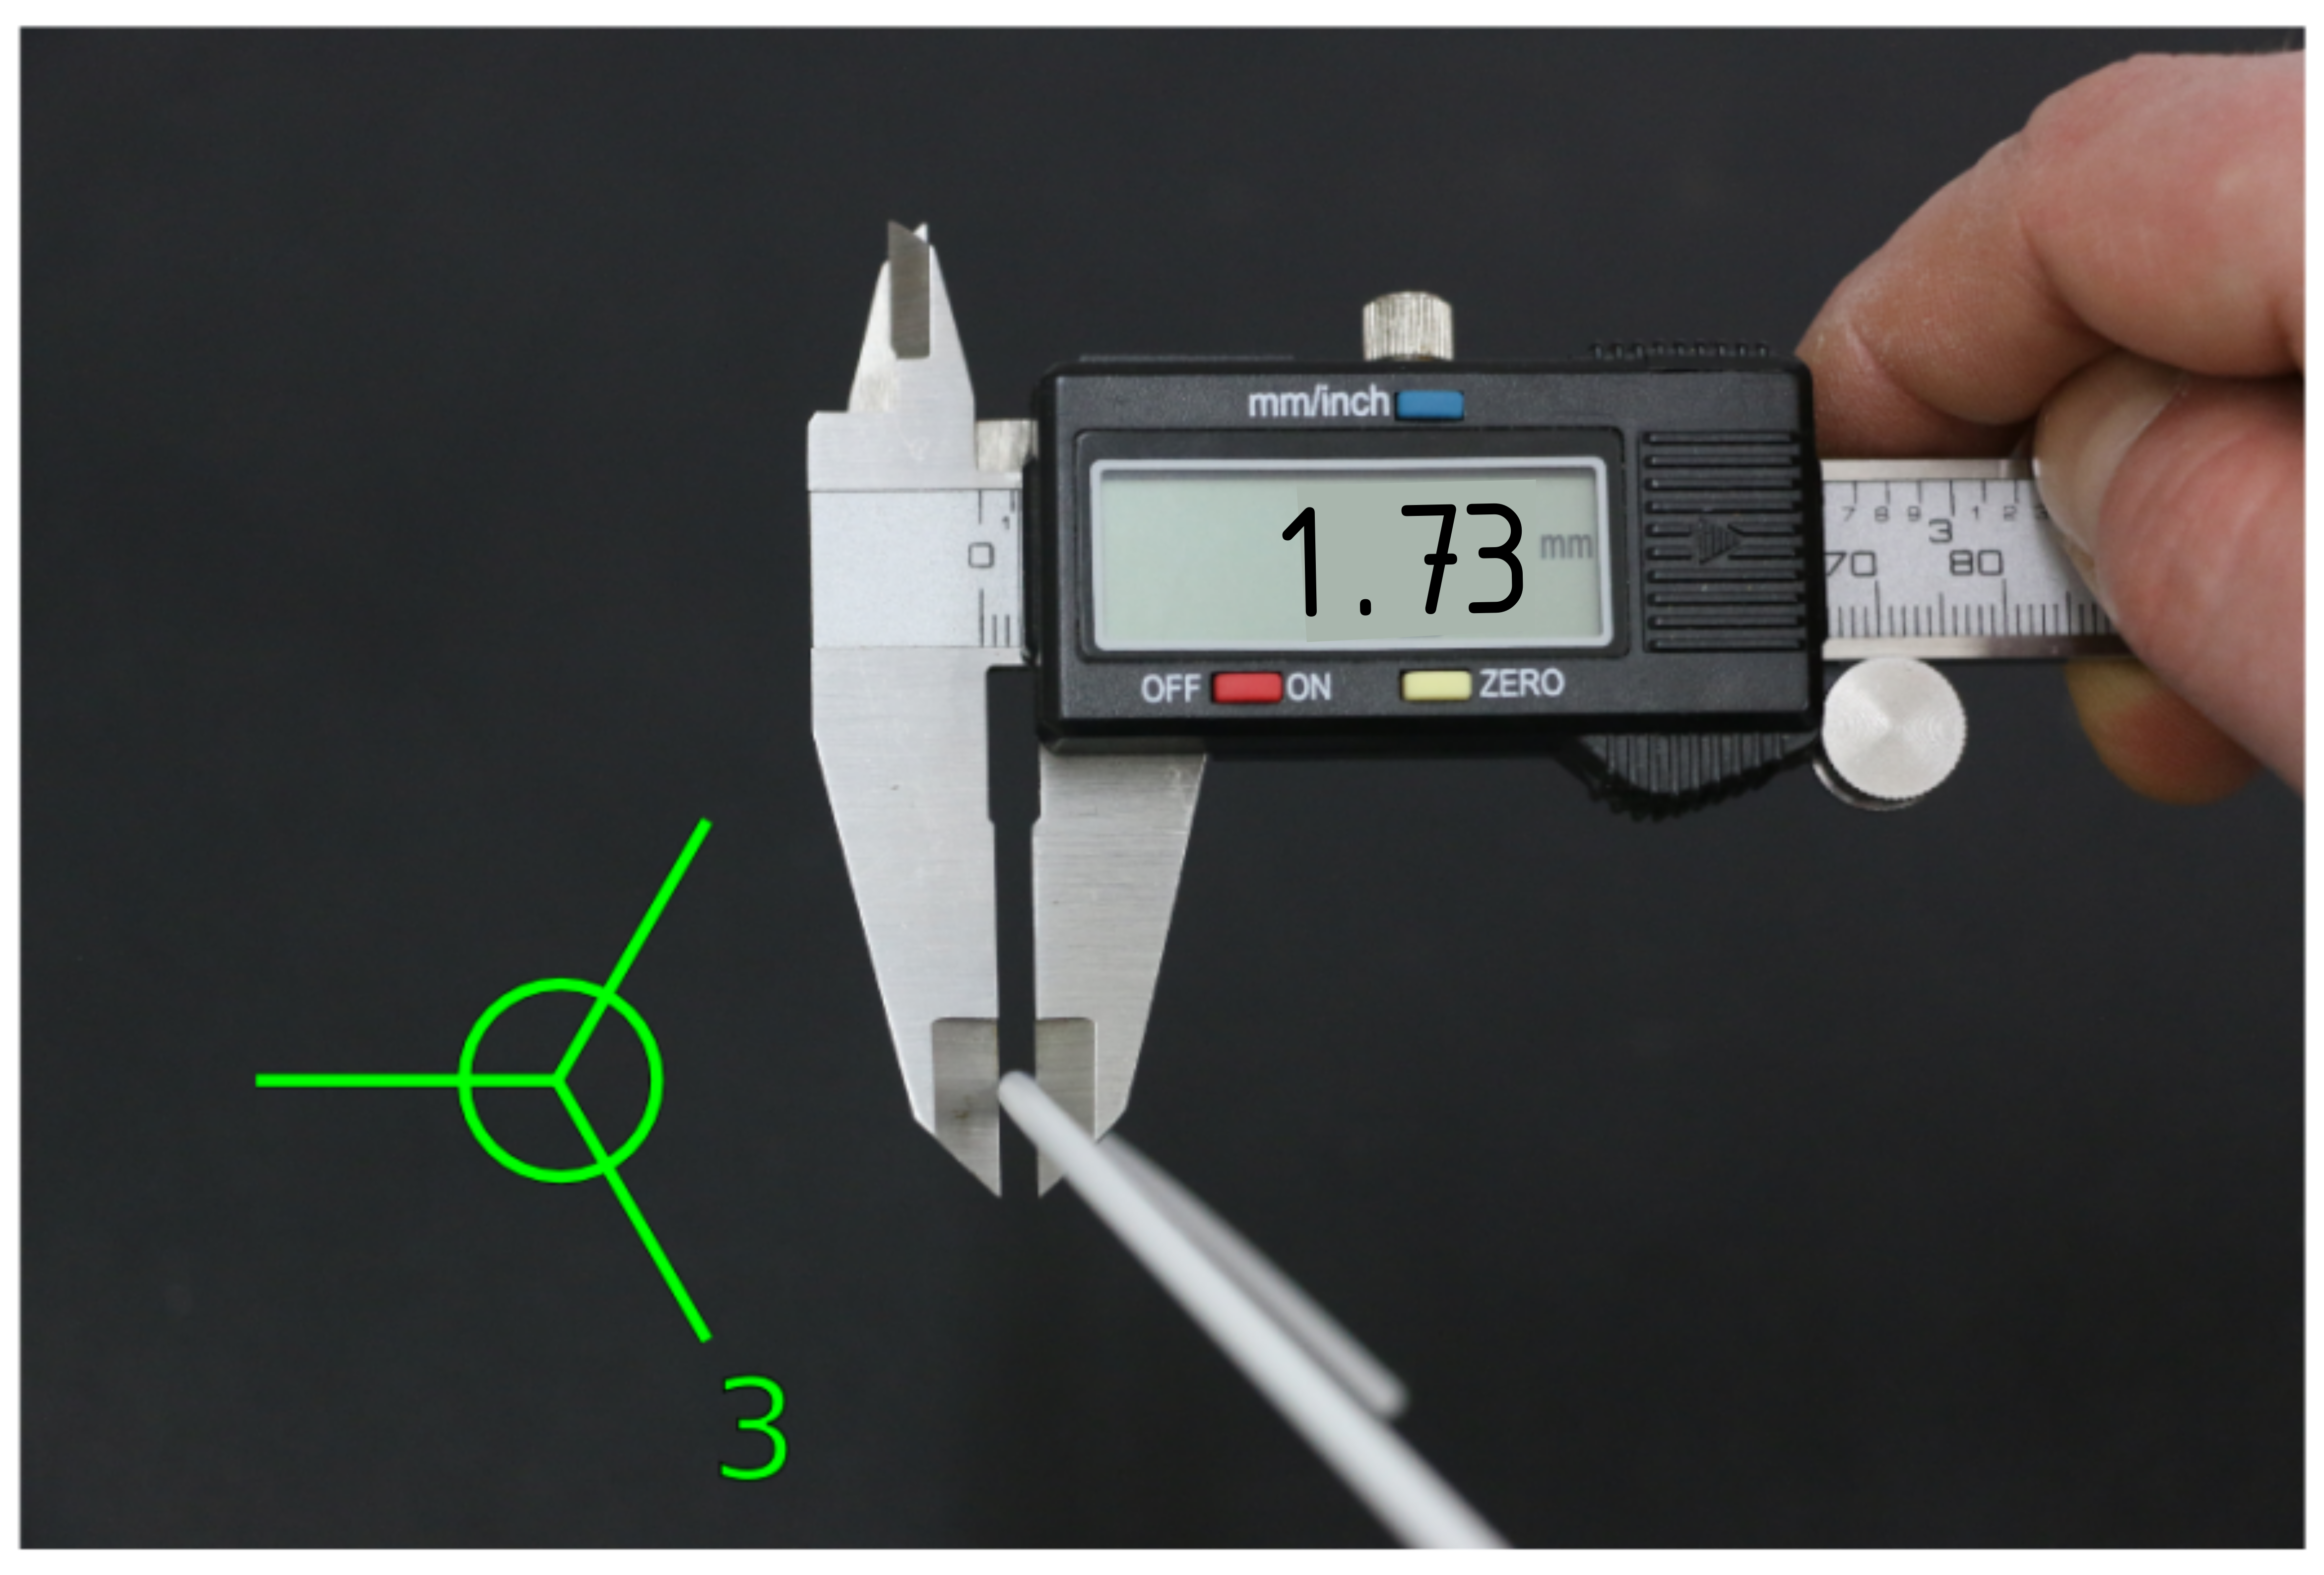
\includegraphics[width=.7\linewidth]{./img/filametmeasurediam_3.png}
  \caption{Third measured diameter - this filament exceeds the stated tolerance and must be 
           replaced.}
\end{figure}


\paragraph{Roundness}

Measure two times at the same point.
If one diameter deviates from the stated tolerance or if both diameters differ strongly, the filament is out of round and must be replaced.

Out of round filament, even when meeting the admissible values, is likely to form a plug inside the nozzle barrel because molten filament can push itself back up past the main strand. 

\begin{figure}[H]
  \centering
  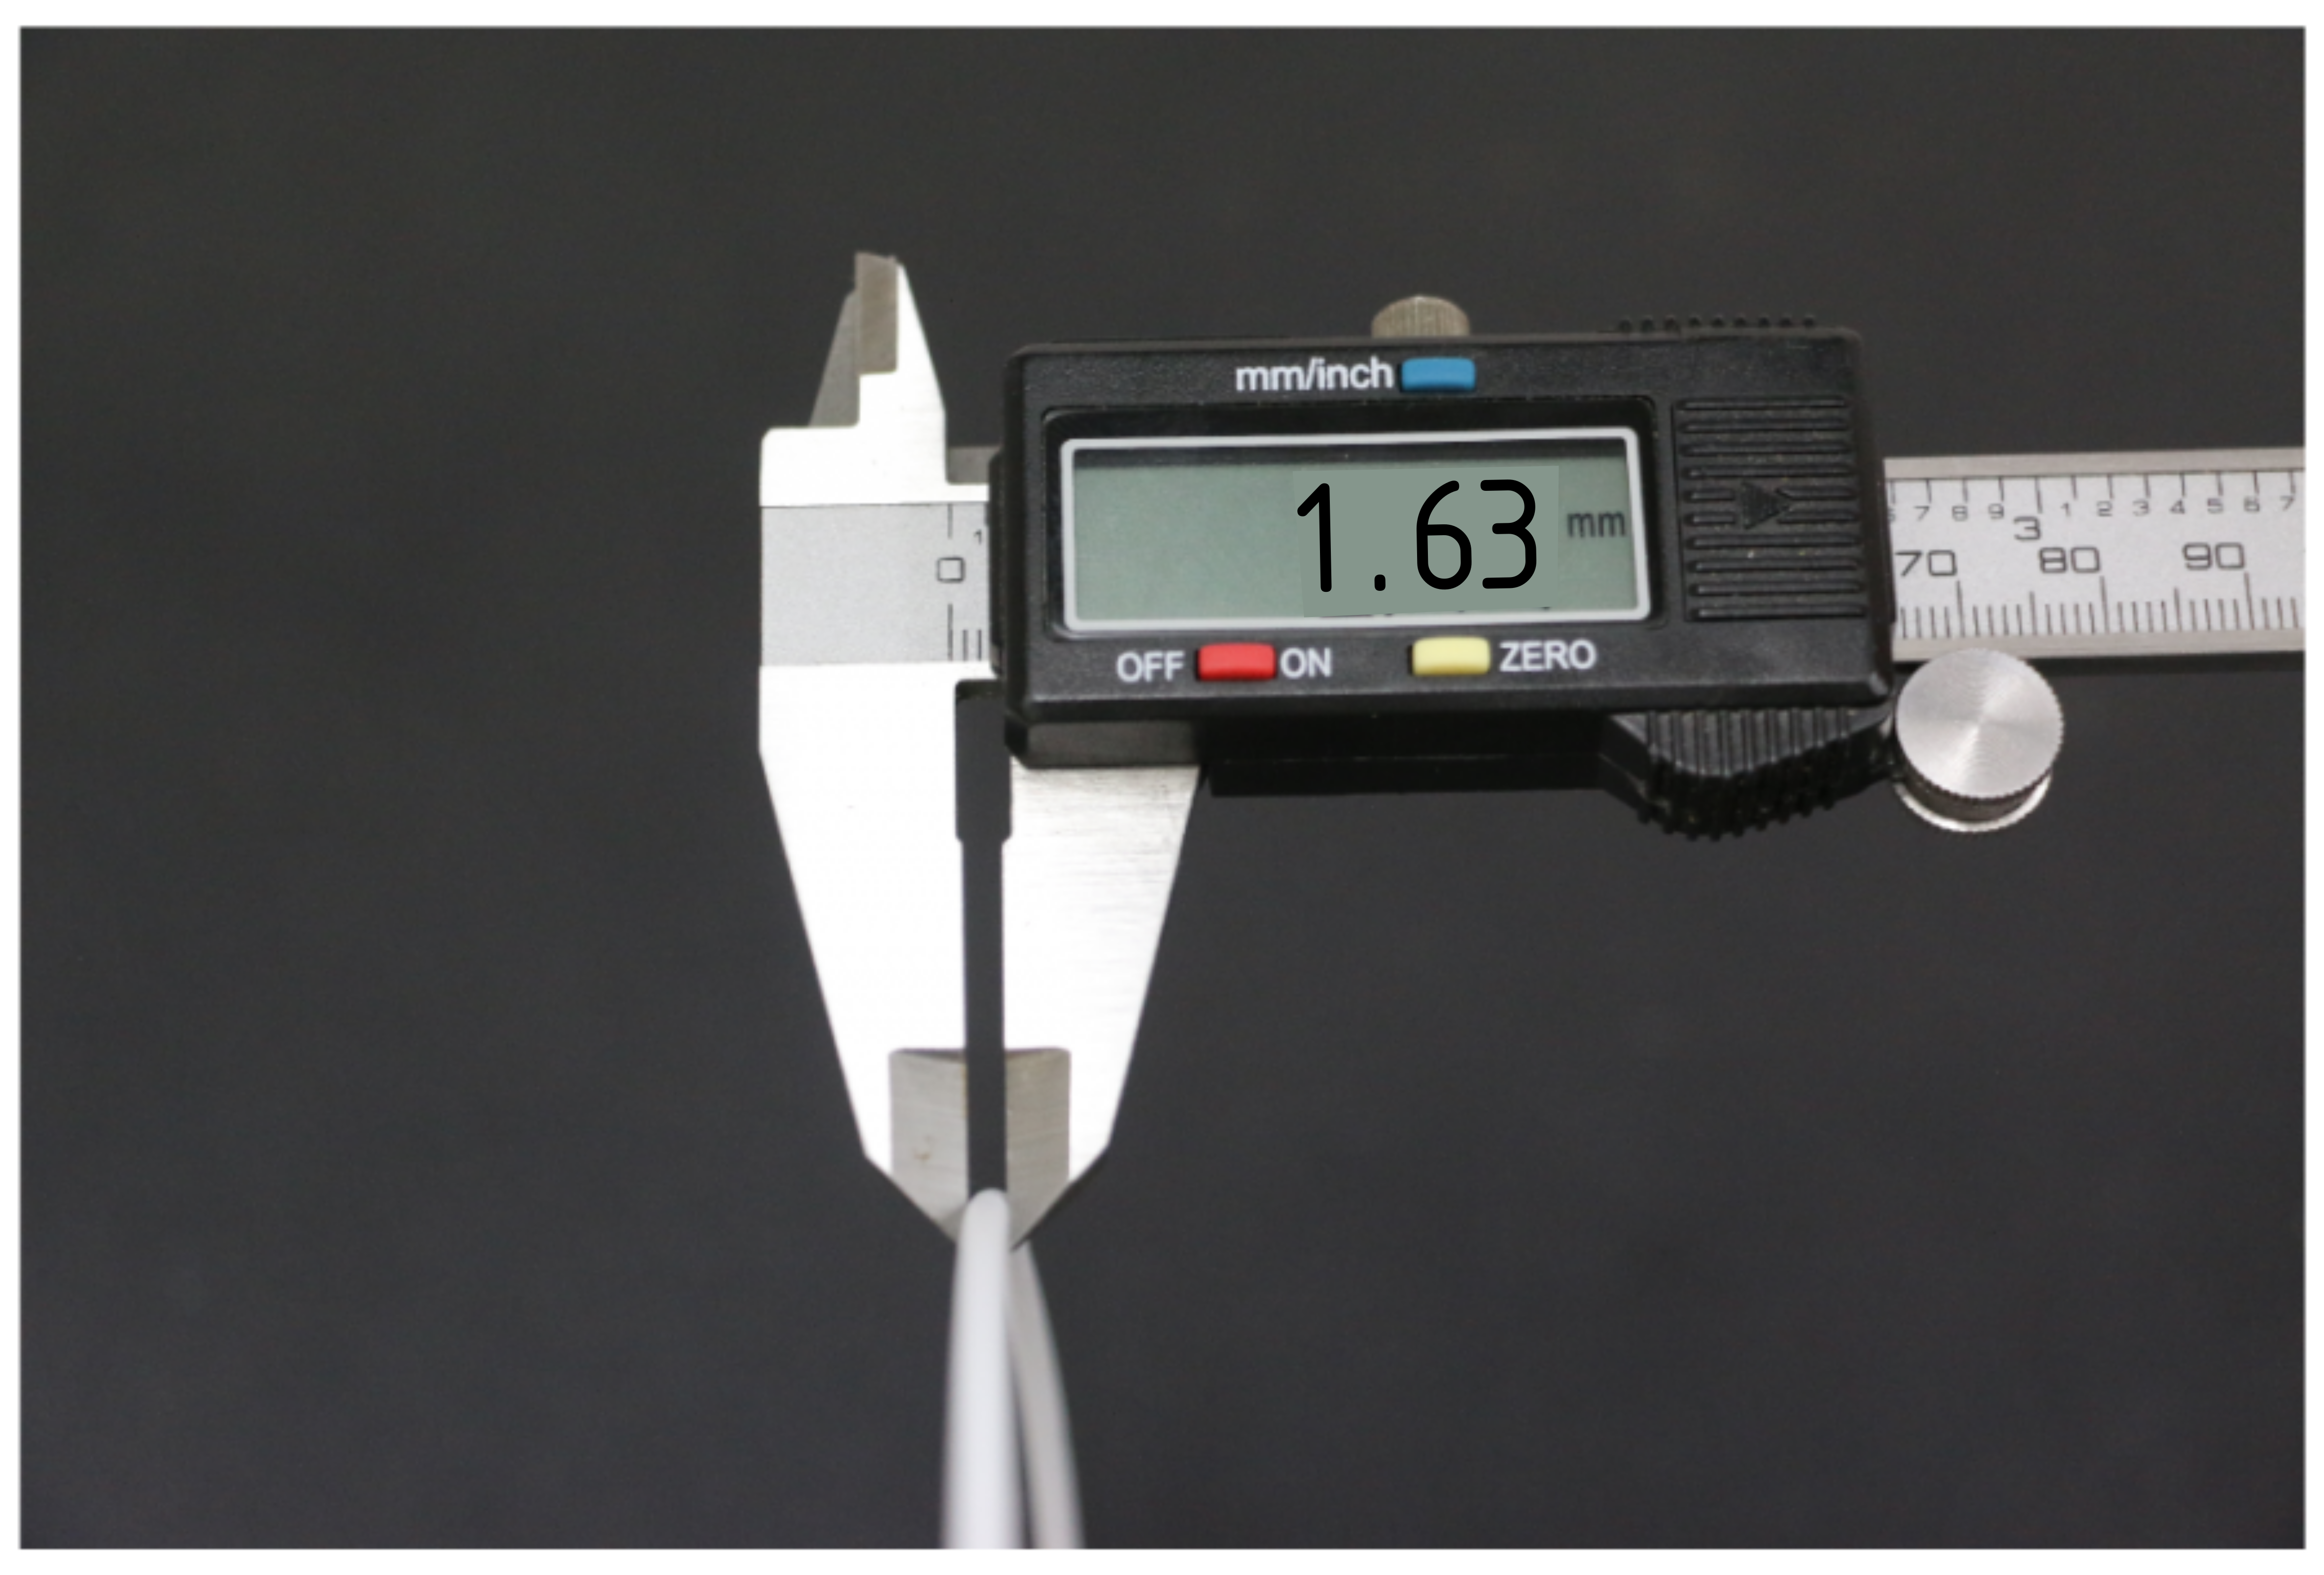
\includegraphics[width=.7\linewidth]{./img/filametmeasureround_1.png}
  \caption{The measured diameter is below the admissible tolerance …}
\end{figure}

\begin{figure}[H]
  \centering
  \includegraphics[width=.7\linewidth]{./img/filametmeasureround_2.png}
  \caption{Measured at the same position, turned 90\degree . The diameter now exceeds the 
           tolerance - the filament is out of round and must be replaced.}
\end{figure}


\paragraph{Kinks and bulges}

Visible quality failure such as kinks or bulges may also increase the friction in the filament feed system. Check for visible deformation. 

\begin{figure}[H]
  \centering
  \includegraphics[width=.7\linewidth]{./img/filametmeasurekinks_1.png}
  \caption{Visible kinks in the filament may also lead to jamming.}
\end{figure}


\subsubsection{Calibrating the extrusion}

The stability and dimensional accuracy of any printed object require a correct amount of filament conveyed through the nozzle. Too little extrusion and the part will be thin-walled, fragile and likely to break. Too much material is likely to clog the nozzle and ruin the print. The amount of material effectively conveyed through the nozzle is depending on: 

\begin{itemize}
  \item the 3D printer itself - slight variations are possible due to the manufacturing 
        process;
  \item the actual filament diameter - in the range of the dimensional stability of the 
        filament;
  \item the printed material's properties - the extruder drive wheel grinds deeper into 
        softer materials, thus reducing the actual diameter;
  \item the idler tension - high tension will cause the drive wheels teeth to grind deeply 
        into the filament, causing a dilation of the material and a reduced output.
\end{itemize}

To make sure that the print result is stable and accurate, an extrusion multiplier must be found for every material on every apparatus; it may be that this factor must be found for every spool of filament.
The correct extrusion multiplier is set in the slicing software, compensating for the above named variables.

To find the correct multiplier, follow the procedure described in the following. The general objective is to print a test part with a known wall thickness dimension, measure the result and calculate the correction factor to compensate any error.

To create a G-code for the extrusion calibration, you need an stl-file of a simple shape (like a cube) - a link to a suitable model can be found in the $\rightarrow$ Downloads section (\ref{sec:downloads}).

\begin{figure}[H]
  \centering
  \includegraphics[width=.7\linewidth]{./img/tt_calibrateextrusion_cubeprepost.png}
  \caption{A simple 30x30x15 mm calibration cube as OpenSCAD model and ready sliced with Slic3r.}
\end{figure}

Load the stl-file in Slic3r and select the \emph{Print Settings} tab.

\begin{figure}[H]
  \centering
  \includegraphics[width=.7\linewidth]{./img/slic3r_selectpartsettings_2.png}
  \caption{Load the calibration cube stl-file in Slic3r.}
\end{figure}

Choose the SOLID profile as a basis.
Choose the following settings to make the cube a box without a lid and only one perimeter of 0.5 mm thickness for a wall: 

\begin{table}[H]
  \centering
  \begin{tabular}{ l l }
    \toprule
    Layers and Perimeters $\rightarrow$ Vertical shells
    Perimeters (minimum) 
      & 1    \\
    Layers and Perimeters $\rightarrow$ Horizontal shells
    Solid Layers TOP 
      & 0    \\
    Layers and Perimeters $\rightarrow$ Horizontal shells
    Solid Layers BOTTOM 
      & 3    \\
    Infill $\rightarrow$ Fill density 
      & 0\%  \\
    Advanced $\rightarrow$ Default extrusion width  
      & 0.5  \\
    Advanced $\rightarrow$ Perimeters
      & 0.5  \\
    Advanced $\rightarrow$ External perimeters
      & 0.5  \\
    \bottomrule
  \end{tabular}
\end{table}

\begin{figure}[H]
  \centering
  \includegraphics[width=.7\linewidth]{./img/slic3r_selectprintsettings_calibrateextrusion.png}
  \caption{Select the Layers and perimeters according to the adjacent table.}
\end{figure}

\begin{figure}[H]
  \centering
  \includegraphics[width=.7\linewidth]{./img/slic3r_selectprintsettingsinfill_calibrateextrusion.png}
  \caption{Select the Infill according to the adjacent table.}
\end{figure}

\begin{figure}[H]
  \centering
  \includegraphics[width=.7\linewidth]{./img/slic3r_selectprintsettings_calibrateextrusion_advanced.png}
  \caption{Select the extrusion widths according to the adjacent table.}
\end{figure}

\begin{info}
  Saving these settings as an “extruder calibration” profile will make this calibration much more comfortable in the future.
\end{info}

Upload the G-code to your 3D printer, print it, measure the wall thicknesses, and calculate the mean value.

The extrusion multiplier is then calculated with the formular (insert your specific measurement):

$$
\frac{expected\ wall\ thickness}{measured\ wall\ thickness} = \frac{0.47 mm}{0.5mm} \approx 1.11
$$

The calculated extrusion multiplier can be entered in Slic3r (Filament settings) and saved in the filament profile. 

\begin{figure}[H]
  \centering
  \includegraphics[width=.7\linewidth]{./img/tt_extrusionmultiplier.png}
  \caption{Enter the extrusion multiplier in Slic3r and 
           save the filament profile (rename!).}
\end{figure}

\subsubsection{Calibrating the extruder offset} \label{sec:offsetcalibration}

For using both extruders of the HT500.3 in one print (see $\rightarrow$ Dual extrusion, section \ref{sec_dualextrusion}) it is vitally important for the machine to know precisely how far both nozzles are offset from each other. To calibrate the extruder offset, a calibration part is printed first. On this part, we can take measurements and input the results into the \emph{Set Extruder Offset} wizard on the machine:

\begin{itemize}
  \item Download the \emph{Extruder Offset Calibration Model} that is linked in the Downloads
        section (see $\rightarrow$ \ref{sec:downloads})
  \item Prepare a bicolored dual extrusion print job from this model like described in sections
        $\rightarrow$ \ref{sec:dualextrusionbasics} and $\rightarrow$ \ref{sec:bicoloredprinting}

  \begin{figure}[H]
    \centering
    \includegraphics[width=.5\linewidth]{./img/calibrate_offset_modeloverview.png}
    \caption{Preparing a calibration print job.}
  \end{figure}

  \item Precisely measure your printed part with calipers to aquire the four measurements as shown here:

  \begin{figure}[H]
    \centering
    \includegraphics[width=.6\linewidth]{./img/calibrate_offset_measurements.png}
    \caption{Measurements to be taken on the printed calibration part.}
  \end{figure}

  \begin{figure}[H]
    \centering
    \includegraphics[width=.4\linewidth]{./img/calibrate_offset_outerdimension.png}
    \includegraphics[width=.4\linewidth]{./img/calibrate_offset_innerdimension.png}
    \caption{Illustration on how to take measurements on the calibration print.}
  \end{figure}

  \item Open the \emph{Set Extruder Offset} wizard in the [Setup] tab on the printer's touchscreen.
  \item Adjust the input mask to match your values for X1, X2, Y1 and Y2.
  \item Tap [Save] to store the updated offset calibration on the printer.
\end{itemize}

\subsection{Dual extrusion} \label{sec_dualextrusion}

\begin{figure}[H]
  \centering
  \includegraphics[width=.7\linewidth]{./img/header_dual_extrusion.png}
  \caption{Excavation finding of the Archeological Institute of the University of Freiburg,
           reprinted on a HT500.3 with black ABS and HIPS as soluble support.}
\end{figure}

\begin{figure}[H]
  \centering
  \includegraphics[width=.7\linewidth]{./img/dual_extrusion_multicolor.png}
  \caption{Things no. 67503 and 318057 from thingiverse.com,
           both printed as multicolor prints in red and white ABS on a HT500.3.}
\end{figure}

One of the HT500.3 3D-printer's core features is its dual extrusion functionality. Producing visually appealing bicolored or bimaterial parts, making functional parts out of a two-material combination or highly accurate complex geometries with fully attached soluble support structures become possible with the two hot-ends extruder head. 

All necessary settings that are required for successfully printing with both hot ends are described in the following.

\subsubsection{Basic dual extruder settings} \label{sec:dualextrusionbasics}

The steps and settings described in the following paragraphs are valid for all multi-material print jobs. Specific information on \emph{printing with soluble support material} or \emph{bicolored} are described in the respective chapters below. 

\paragraph{3D printer preparation}

Depending on the task, the setup of the 3D printer for dual extruder prints may vary.
Printing bicolored objects will mostly be done with the same resolution requirements throughout the print, so installing the same nozzle diameter on both hot ends is recommended.
For printing support structures with a second material, printing the support with a larger nozzle helps reducing printing time since the printing resolution of the support is not vital for the appearance. Slic3r will calculate interface layers accordingly for nevertheless satisfying results.
Make sure to have installed the nozzle suited to the task on each hot end, and that they are precisely leveled. Compare your setup with your Slic3r settings and adjust these if necessary.

Perform each of the calibrations once before the first print. The settings may remain unchanged if no hardware changes (i.e. nozzle exchange) are made.  

\begin{enumerate}
  \item For dual extruder prints it is vitally important that both hot ends are precisely 
        leveled to the same height. If not yet done, run the [Print Bed Leveling] wizard and follow the on-screen instructions.
  \item The offset of the hot ends must also be calibrated to ensure accurate relative
        positioning. Run the Extruder Offset Calibration Routine as described in section \ref{sec:offsetcalibration}
  \item Do not forget to check the extrusion multiplier for the installed materials and 
        respectively to run the [Calibrate Extrusion] wizard for each hot end if required.
\end{enumerate}

\begin{figure}[H]
  \centering
  \includegraphics[width=.7\linewidth]{./img/header_dual_extrusion_leveling.jpg}
  \caption{Precise leveling of both hot ends is mandatory for dual extruder prints.}
\end{figure}

The 3D printer hardware is now ready for dual extrusion. 

\paragraph{Wiper check}

Check that the wiper lip and the nozzle tips are aligned correctly: 

\begin{itemize}
  \item Open the \emph{[Expert Control]} screen and move the print head to 
        the maintenance position.
  \item Move the left nozzle so that it rests directly behind the wiper lip.
  \item Make sure the lip's upper rim is aligned in the middle of the nozzle's conical tip 
       (see adjacent picture). Adjust the wiper lip if required.
  \item Home the print head.
\end{itemize}


\begin{info}
  The nozzles must be precisely leveled to the same height.
\end{info}

\begin{figure}[H]
  \centering
  \includegraphics[width=.7\linewidth]{./img/wiper_align.png}
  \caption{Nozzle cone and wiper lip are correctly aligned.}
\end{figure}

All necessary settings to effect the required movement of the print head into a g-code are implemented in the \emph{Tool change G-code} in the \emph{Custom G-code} menu 
of Slic3r's \emph{Printer Settings}. It is only filled in when one of the 
\emph{Dual Extruder} profiles has been chosen.

\begin{figure}[H]
  \centering
  \includegraphics[width=.7\linewidth]{./img/slic3r_printer_toolchangegcode.png}
  \caption{The Slic3r tool change G-code provides the information for the wiping process. 
           It is preconfigured and normally does not need interference.}
\end{figure}

\paragraph{Slic3r presets}

The full usability of the dual extrusion function is highly depending on the slicing software. As always, Kühling\&Kühling recommend using Slic3r Prusa Edition.
The Slic3r-profile at our GitHub repository (see $\rightarrow$ \emph{Downloads} in section \ref{sec:downloads}) already come with tested and recommended presets for dual extrusion. 

To begin with dual extruder printing the easiest way is to choose the respective preset in in the \emph{Plater} menu of Slic3r: 

\begin{figure}[H]
  \centering
  \includegraphics[width=.7\linewidth]{./img/slic3r_dualex_plater.png}
  \caption{Preselecting in Slic3r for dual extruder printing.}
\end{figure}

\begin{enumerate}
  \item \emph{Print settings} \newline
    for the extrusion, there is no difference between single and dual extruder prints; choose \emph{SOLID, ECO} or \emph{SOLID (soluble support)}
    according to your needs. \newline
    Regard that the extruder nozzles must be \emph{assigned correctly}.

  \item \emph{Printer} \newline
    from the printer profiles select
    \emph{DUAL EXTRUDER (bicolored, nozzles 0.35+0.35)} \newline
    or
    \emph{DUAL EXTRUDER (soluble support, nozzles 0.35+0.5)} 
    according to the task. \newline
    After choosing either dual extruder profile a second \emph{Filament} dropdown menu appears.

  \item \emph{Filament}
    Choose the material type for each extruder individually. The first (upper) material is selected for the left extruder, 
    the second (lower) is selected for the right extruder. \newline
    Regard that a second material can only be chosen after dual extrusion has been selected in the \emph{Printer} dropdown menu. \newline
    Additional information on well-functioning combinations of materials can be found in the chapter \emph{materials}.
\end{enumerate}

Upload your 3D model and adjust all necessary settings as usual.
For \emph{supported prints} no further manipulation of the 3D model is required.
For \emph{bicolored prints} additional preparations are necessary. 

\subsubsection{Printing with soluble support material}

Common break-away support is not what takes 3D printing to its limits since its flaws nearly void the possibilities when it comes to surface quality. Due to the necessary gap between support structure and model underside, the later are always subject to gravity and will sag a little, reducing the contact to following layers. To really produce optically impeccable undersides a closely fitting, gapless support is required.
For printing with a soluble support material, it is mandatory that the slicing software provides the possibility of defining the distance between support and model. Only if no gap remains between these two, the superiority of soluble support compared to break-away structures becomes visible in the model.

The following Slic3r presets are provided with 
the Kühling\&Kühling printing profile \emph{SOLID (soluble support)}. This description is meant to give you all necessary information to try out new settings. 

\begin{itemize}
  \item Menu “Print Settings” 

  \begin{itemize}
    \item \emph{Layers and perimeters}

      \begin{itemize}
        \item The \emph{First layer height} must match the diameter of 
              the support material extruder (the right extruder is preset). 
      \end{itemize}

      \begin{info}
        This function cannot be used with any ECO profile or similar settings because the solvent for the support material may soak into the model which can cause long-term damage.
      \end{info}

      \begin{figure}[H]
        \centering
        \includegraphics[width=.7\linewidth]{./img/slic3r_bicolor_new2.png}
        \caption{First layer height and support material extruder nozzle diameter
                 must correspond.}
      \end{figure}

    \item \emph{Support material} 

      \begin{itemize}    
        \item The checkbox \emph{Generate support material} must be activated. If required, 
              the \emph{Overhang threshold angle} can be adjusted accordingly 
              (check via the \emph{Preview} in the \emph{Plater}).
        \item The \emph{Contact Z distance} must be “0 (soluble)” with a (recommended) 
            “rectilinear” \emph{Pattern} and a \emph{Pattern spacing} of 1.25 mm.
        \item It is a good idea to generate \emph{5 - 7 Raft} layers with 
              the support material. 
              Thus, slight leveling mistakes are compensated and an even and reliable subsurface is always provided.
      \end{itemize}

	  \begin{figure}[H]
        \centering
        \includegraphics[width=.7\linewidth]
           {./img/slic3r_printsettings_supportmaterial_z0.png}
        \caption
           {Choose these settings for dual extruder prints with soluble support material.}
      \end{figure}

    \item \emph{Multiple Extruders $\rightarrow$ Extruders}

      \begin{itemize}
        \item Select the model and the support extruder according to the 
              loaded materials. \newline
              Preset recommendation: \newline
              \emph{Perimeter/Infill/Solid infill extruder} $\rightarrow$ Extruder 1
              \emph{Support material/raft/skirt/interface extruder} $\rightarrow$ 
              Extruder 2.  
      \end{itemize}

      \begin{figure}[H]
        \centering
        \includegraphics[width=.7\linewidth]{./img/slic3r_multipleextr_12.png}
        \caption{Assigning the hot ends to their respective tasks.}
      \end{figure}
    
  \end{itemize}

  \item Menu “Printer Settings”
  
  \begin{itemize}
    \item \emph{Extruder 1 / Extruder 2 $\rightarrow$ Size} 

        \begin{itemize}
          \item Check that the correct nozzle size is set for each extruder 
               (remember the \emph{First layer height}). 
        \end{itemize}


      \begin{figure}[H]
        \centering
        \includegraphics[width=.7\linewidth]{./img/slic3r_multipleextr_e1e2.png}
        \caption{Make sure the correct nozzle size has been entered for each extruder.}
      \end{figure}

  \end{itemize}

\end{itemize}

\subsubsection{Post-treatment of soluble HIPS support}

\begin{danger}
  d-limonene is very toxic to aquatic organisms and must not enter the sanitation.
  Make sure to dispose of d-limonene in a suitable and environmental friendly way.
  Regard the manufacturer's safety data sheet when handling d-limonene. 
\end{danger}

\begin{danger}
  d-limonene and its fumes are flammable.
  Do not handle in the vicinity of heat, open flames, hot surfaces and other ignition sources.
  Do not smoke.
  Regard the manufacturer's safety data sheet when handling d-limonene. 
\end{danger}

\begin{danger}
  d-limonene is a solving agent and therefor must not be handled carelessly.
  d-limonene can cause skin and eye irritations.
  Wear suitable protective gloves and goggles and regard the manufacturer's safety data sheet when handling d-limonene. 
\end{danger}

After a complex ABS model has successfully been printed with HIPS soluble support material, the support material must be removed and dissolved. This is an easy process that only requires only a few steps:

\begin{itemize}
  \item Mechanically break away the easily accessible parts of the support material.
  \item Place the model in a bath of Kühling\&Kühling wash-out solution (97\% d-limonene - 
        order directly via sales@kuehlingkuehling.de) so that it is fully submerged. The bath is best stirred, either with a magnetic stirrer or by other means to provide its full solving capacity and to reduce bathing time.
  \item When all remaining HIPS has been dissolved (check occasionally) remove the model 
        from the bath, briefly dry it with a paper towel, and leave it in a warm and bright place (e.g. windowsill) to dry completely.
\end{itemize}


\subsubsection{Bicolored printing} \label{sec:bicoloredprinting}

\begin{figure}[H]
  \centering
  \includegraphics[width=.7\linewidth]{./img/cat_split.png}
  \caption{3D model preparation for bicolored printing example 1:
           a model (http://www.thingiverse.com/thing:62536) split in two for bicolored printing. Both must be aligned with the same relative position and exported as separate STLs.}
\end{figure}

\begin{figure}[H]
  \centering
  \includegraphics[width=.7\linewidth]{./img/cat_merged.png}
  \caption{The two parts correctly positioned and ready for export.}
\end{figure}

\begin{figure}[H]
  \centering
  \includegraphics[width=.7\linewidth]{./img/slic3r_bicolor_1.png}
  \caption{3D model preparation for bicolored printing example 2: both individual parts 
           of the 3D model being aligned in a common assembly and exported as separate STL-files with the correct relative coordinates.}
\end{figure}

The model preparation for bicolored (and also multi-material) prints is somewhat more complex than supported prints since Slic3r cannot distinguish single areas of a certain model and therefor is not able to automatically calculate the necessary commands. The respective 3D model must be designed as two separate parts with exact relative coordinates to enable Slic3r positioning them as required.

It is best to create the model from two separate parts and join and position them in a common assembly before exporting each as STL, so that the relative positions are recorded in the individual files. Slic3r has the feature to combine multiple STL files into a multi-material print job. Split the original design into the separate parts within the CAD program, and export each part as STL. Make sure both parts do not intersect. 

Uploading and slicing the parts: 

\begin{itemize}
  \item Upload the first part to the \emph{Plater}.
  \item Open the \emph{Settings} dialog.
 
  \begin{figure}[H]
    \centering
    \includegraphics[width=.7\linewidth]{./img/slic3r_bicolored_cat1.png}
    \caption{The first part is loaded to the Plater directly.}
  \end{figure}
  
  \item Mark part one and assign it to extruder \emph{1}.
  \item Click \emph{Load part …} and add the second part from your file system.
        If the single parts are aligned correctly, the preview should now show the exact representation of your desired model.

  \begin{figure}[H]
    \centering
    \includegraphics[width=.7\linewidth]{./img/slic3r_bicolored_cat2.png}
    \caption{After the extruder for the first part has been assigned, 
             the second part is loaded via the Settings dialog.}
  \end{figure}

  \item Mark the second part and assign to extruder \emph{2}.
  \item Close the settings by clicking \emph{OK}.

  \begin{figure}[H]
    \centering
    \includegraphics[width=.7\linewidth]{./img/slic3r_bicolored_cat3.png}
    \caption{The second part must be assigned to extruder 2.}
  \end{figure}


  \item You can add and load more than one part and modify it as described above.
  \item Adjust all other necessary settings as usual 
        and as described in Basic dual extruder settings.
  \item Prepare the 3D printer as described in 3D printer preparation.


  \begin{figure}[H]
    \centering
    \includegraphics[width=.7\linewidth]{./img/slic3r_bicolored_cat4.png}
    \caption{This is what the preview should look like: both parts clearly 
             visible in their correct position.}
  \end{figure}

\end{itemize}

\subsection{Tips \& Tricks}

Here you will find information about issues concerning the operation of the HT500.3 in your specific work environment or solutions for questions that have been upraised by support requests. 


\subsubsection{Commandline Access to the linux operating system via SSH} \label{sec:commandlineaccess}

Use SSH on your computer connected to the same LAN as your 3D printer to log in to the HT500.3's built-in Linux computer. You can use the hostname from the printers' 
\emph{Backend-URL} and log in with the following access data: 

\begin{verbatim}
User: kiosk
Password: eight-digit combination from the serial number at the back
  of the device. Take the first two four-digit blocks,
  XX-AAAA-BBBB-CCCC-YYYY becomes an "AAAABBBB" password.
\end{verbatim}


\subsubsection{Setting a static IP address for HT500.3 ethernet connection}

First, establish a commandline connection to the printer ($\rightarrow$ section \ref{sec:commandlineaccess}). 
From within the terminal session, you can edit the system's network configuration via the command line editor “nano”.

\begin{verbatim}
sudo nano /etc/network/interfaces
\end{verbatim}
The current DHCP setup looks like:
\begin{verbatim}
\# The primary network interface
auto eth0
iface eth0 inet dhcp
 pre-up iptables-restore </etc/iptables.rules

Change the setup according to your needs. Example:

  \# The primary network interface
  auto eth0
  iface eth0 inet static
  address 192.168.1.20
  netmask 255.255.255.0
  broadcast 192.168.1.255
  gateway 192.168.1.1
  dns-search family.local
  dns-nameservers 192.168.1.1
    pre-up iptables-restore </etc/iptables.rules
\end{verbatim}
The rest of the file remains unchanged. Save the file using CTRL+X and confirm the overwrite query with “Y”. Disconnect and finish by typing
\begin{verbatim}
exit
\end{verbatim}
Shut down and reboot the HT500.3 to establish the alterations.

\subsubsection{Use a custom NTP server for time signals}

First, establish a commandline connection to the printer ($\rightarrow$ section \ref{sec:commandlineaccess}).

From within the terminal session, stop the NTP daemon background process
\begin{verbatim}
sudo service ntp stop
\end{verbatim}
Edit the NTP daemon configuration via the command line editor “nano”
\begin{verbatim}
sudo nano /etc/ntp.conf
\end{verbatim}
Search for the few lines beginning with
\begin{verbatim}
server ...
\end{verbatim}
and add an additional new line before these with the address to your local NTP server like this
\begin{verbatim}
server 192.168.1.123
\end{verbatim}
add another additional statement anywhere in this file
\begin{verbatim}
# ignore panic threshold for huge time differences
tinker panic 0
\end{verbatim}
The rest of the file remains unchanged. Save the file using CTRL+X and confirm the overwrite query with “Y”.\\
Re-enable NTP client service for background operation
\begin{verbatim}
sudo service ntp start
\end{verbatim}
Disconnect and finish by typing
\begin{verbatim}
exit
\end{verbatim}
\emph{Shut down} and \emph{reboot} the HT500.3 to establish the alterations. 


\subsubsection{Changing Shell Password in the Linux Operating System}

After manually creating a new Micro-SD Card from a pre-packaged upgrade release provided by Kühling\&Kühling, the user account running the RepRapOnRails software in the Linux operating system will be in default configuration. To change the password, use SSH on your computer connected to the same LAN as your 3D printer to log in to the operating system. You can use the hostname in the printers' \emph{Backend-URL} as its address and log in with the following access data:
\begin{verbatim}
User: kiosk
Password: kiosk
\end{verbatim}
Now you can set a new password by entering
\begin{verbatim}
passwd
\end{verbatim}
and following the instructions. In delivery condition the unique password is an eight-digit combination from the serial number at the back of the device. Take the first two four-digit blocks (example: XX-AAAA-BBBB-CCCC-YYYY becomes an “AAAABBBB” password). 


\subsubsection{Print bed leveling}

Accurate leveling is vitally important for the print result. Although correct first layer settings can compensate for slight unevennesses of the print bed, false leveling will ruin a print within the first few layers.
Evidence for a leveling mistake can be:

\begin{table}[H]
  \centering
  \begin{tabulary}{\textwidth}{ L L L }
    \toprule
    No.  
      & Appearance 
        & Reason       \\
    \midrule
    1   
      & Asymmetrical layer thickness, especially of the first layer.  
        & lopsided leveling
          Appearance 2 and 3 are visible simultaneously   \\
    2   
      & Smearing of the extrusion and possibly clogging of the nozzle.  
        & Print bed and the nozzle are too close together. \\
    \multirow{2}{*}{3}   
      & The extruded strand is laid on the print bed instead of being spread.   
        & Print bed and the nozzle are too far apart.      
          (can be due to a wrong bed temperature also – better double-check) \\
      & Strands do not stick to the print bed but are being pulled away by the nozzle tip.
        &                 \\
    4  
      & Extrusion of rounded, unjoined strands.   
        & Print bed and the nozzle are too far apart. \\
    \bottomrule
  \end{tabulary}
\end{table}

\begin{figure}[H]
  \centering
  \includegraphics[width=.7\linewidth]{./img/lopsidedleveling.png}
  \caption{Leveling mistakes: examples of characteristic appearances of the first layer.}
\end{figure}

To avoid such irritations, make use of the following tips: 

\begin{itemize}
  \item Always make sure that the build chamber is adequately and uniformly preheated to of the target
        temperature.
        The Z-end stop is temperature sensitive and may cause deviating positioning when exposed to temperature variations.
        Keep the build chamber doors as shortly open as possible during leveling to avoid too much heat loss.
  \item If you removed the print bed, always re-insert it in the same direction and 
        orientation it had during leveling.
  \item Put the print bed with the convex side down onto the print table.
  \item After adjusting all three leveling points, return the print head to the first 
        position (tap the \emph{[Back]} button). Check the bed - tip distance by tapping 
        (\emph{not} pressing) the print bed with a finger next to the nozzle tip: if you see a gap appearing at the slightest touch, the leveling point is correctly adjusted. If even the least pressure is required, the leveling is too high. Repeat this at the other two leveling points. Have a look at the adjacent videos for visual explanation.
  \item Before waisting time on unsuccessful leveling, please rethink if the currently 
        installed nozzle tip is adequate for the print job. Wider nozzles are more tolerant when it comes to compensating leveling mistakes and may be more suited to the task, especially when printing larger parts.
\end{itemize}


\paragraph{Tips for easier bed leveling}

If you find it difficult to adjust the three leveling points uniformly with only the spring pressure, place a sheet of paper (not more than standard 80 g/m\textsuperscript{2}) between the nozzle tip and the print bed and carefully push the bed against the tip before fastening the set screws. This way, you ensure a uniform bed - tip distance at all three leveling points.

\begin{figure}[H]
  \centering
  \includegraphics[width=.7\linewidth]{./img/levelingpaperspacer.jpg}
  \caption{Manual leveling with paper spacer.}
\end{figure}

Another way of making leveling a little bit less important is “floating” your print on a raft. Slic3r (and most other slicing software) provides the “raft” function, a special kind of support material, which means that before starting with the actual object a (customizable) number of loosely printed layers is printed to compensate slight leveling mistakes. If you choose the raft settings correctly, beginning with a layer as wide and thick as allowable (depending on the nozzle tip's diameter) leveling will become a much less delicate process.

The raft's first layer is treated as the print's first layer and uses the respective settings. The following layers of the raft are calculated according to the support material settings. Choose the maximal first layer height 
(Slic3r $\rightarrow$ Print Settings $\rightarrow$ Layers and perimeters/First layer height) and a first layer extrusion width of 250\% 
(Slic3r $\rightarrow$ Print Settings $\rightarrow$ Advanced/Extrusion width -First layer) for a compensating, condoning and stable raft.
The raft can either be built of the model's material and cut away later or, if available for the specific plastic, of support material and broken off or dissolved. For break-away or soluble rafts the dual extrusion function of the HT500.3 is required. Remember to check that all necessary calibrations and settings have been made as described above. 

\begin{figure}[H]
  \centering
  \includegraphics[width=.7\linewidth]{./img/slic3r_adding_raft_layers.png}
  \caption{Adding a freely choosen number of raft layers to the print.}
\end{figure}


\subsubsection{Deactivating the heating elements after end of print job}

Sometimes you may want to start a print job just before finishing time or the weekend. Since there is currently no automatic shutdown function, the 3D printer will then stay on all night respectively some days. With the following description you can alter the End G-code of your print so that the heating elements are shut off after the print job has been finished so that the power consumption is reduced significantly. A side effect is, that due to the fact that the build chamber needs some hours to channel off the heat the cooling process is slowed and thereby internal tensions of the printed object are reduced. To deactivate the heating elements after a print job: 

\begin{enumerate}
  \item Start your slicing software.
  \item Open the [Printer Settings] tab.
  \item Choose the “Custom G-code” menu.
  \item In the End G-Code editor scroll down to the end of the text field and position the 
        cursor in the last line above the \verb|; /END-GCODE| entry.
  \item Enter the command\\
        \verb|M104 S0 T2|\\
        This will set the heating elements of the build chamber to a 
        temperature of 0\degree C.
  \item Enter the command\\
        \verb|M140 S0|\\
        This will deactivate the print bed as the last action of the current G-code.
\end{enumerate}

\begin{figure}[H]
  \centering
  \includegraphics[width=.7\linewidth]{./img/tt_slic3r_modify_endgcode_autooff.png}
  \caption{Switching off the build chamber heating elements by modifying the Slic3r 
           custom End G-code.}
\end{figure}

\subsubsection{Adjusting the build chamber temperature}

\begin{notice}
  The build chamber temperature is preset to the maximal permissible temperature 
  of +70\degree C at delivery.
  Exceeding +70\degree C will damage interior components of the HT500.3 such as stepper motors, bearings and electronics.
\end{notice}

Since an actively heated build chamber is still rare among commercially available 3D printers, common slicing software does not feature ambient temperature settings. For some materials, it is advantageous to modify the chamber temperature together with the other temperature settings. The build chamber's temperature of the HT500.3 is set via the “Start G-code” which can be manually altered.

To change the build chamber temperature (in the following example we use our standard 
\emph{Slic3r} - other software may differ in denotations):

\begin{enumerate}
  \item Open your slicing software.
  \item Open the tab [Printer Settings].
  \item Choose the \emph{Start G-code} editor in the “Custom G-code” menu.
  \item Scroll down to\\
        \verb|; PREHEAT BED AND CHAMBER|
        and position the cursor in the line reading:\\
        \verb|M104 S70 T2; set recirculating air heater to 70 degree celcius target temperature|
  \item Change the entry \verb|“Sxy”| (here \emph{S70}) by replacing the value xy with the desired 
        temperature, for example 50\degree C:\\
        \verb|M104 S50 T2; set recirculating air heater to 50 degree celcius target temperature|\\
        (for logical reasons, the comment should be aligned).
  \item If you want to keep the settings, save them in a new profile 
        (see \emph{Slic3r manual}).
\end{enumerate}

\begin{figure}[H]
  \centering
  \includegraphics[width=.7\linewidth]{./img/tt_slic3r_modify_startendgcode.png}
  \caption{Changing the build chamber temperature by modifying the Slic3r custom Start 
           G-code.}
\end{figure}

Any G-code exported with this profile loaded will heat the build chamber to the stated temperature prior to printing. 


\subsubsection{G-code manipulation at the GUI}

The following list contains supported G-code commands that can be used on demand to directly interfere with a print procedure or setting via the G-code keyboard of the GUI's 
\emph{Log} menu. 

\begin{figure}[H]
  \centering
  \includegraphics[width=.7\linewidth]{./img/tt_gui-loggcodekeys.png}
  \caption{The G-code keyboard in the Log menu provides all keys to enter G-code commands.}
\end{figure}

\begin{table}[H]
  \centering
  \begin{tabulary}{\textwidth}{ L L L }  
    \toprule
    Command   
      & Effect  
        & Example     \\
    \midrule
    G1  
      & Coordinated Movement X Y Z E  
        & G1 X130 Y85 Z1.75 E4.35     \\
    G4 S<seconds>   
      & Wait for given duration in seconds  
        & G4 S5 (waits 5 seconds)  \\
    G28   
      & Home all axes 
        &        \\
    G90   
      & Use absolute coordinates 
        &       \\
    G91   
      & Use relative coordinates 
        &       \\
    M80  
      & Activate build chamber  
        &      \\
    M82   
      & Set E codes absolute (default)
        &       \\ 
    M83   
      & Set E codes relative while in Absolute Coordinates (G90) mode
        &         \\
    M104 S<temp> T<extruder>  
      & Set temperature without wait  
        & \emph{Adjusting the build chamber temperature,
               Deactivating the heating elements after end of print job}     \\
    M109 S<temp> T<extruder>  
      & Set temperature with wait  
        &       \\
    M140 S<temp>  
      & Set bed target temp without wait 
        &       \\
    M190 S<temp>  
      & Set bed target temp with wait   
        &      \\
    M221 S<extrusion flow multiplier in percent>  
      & Increase/decrease given flow rate   
        & M221 S95     
          $\rightarrow$ decrease flow to 95\% of g-code value     \\
    M220 S<print speed multiplier in percent>   
      & Increase/decrease print speed of all drive speeds   
        & M220 S95     
          $\rightarrow$ decrease print speed to 95\% of g-code value      \\
    \bottomrule
  \end{tabulary}
\end{table}